% Based on the resources listed below.
% Joseph Van Boxtel, Daniel Brown, Jakob Miner
%
%Copyright 2014 Jean-Philippe Eisenbarth
%This program is free software: you can
%redistribute it and/or modify it under the terms of the GNU General Public
%License as published by the Free Software Foundation, either version 3 of the
%License, or (at your option) any later version.
%This program is distributed in the hope that it will be useful,but WITHOUT ANY
%WARRANTY; without even the implied warranty of MERCHANTABILITY or FITNESS FOR A
%PARTICULAR PURPOSE. See the GNU General Public License for more details.
%You should have received a copy of the GNU General Public License along with
%this program.  If not, see <http://www.gnu.org/licenses/>.

%Based on the code of Yiannis Lazarides
%http://tex.stackexchange.com/questions/42602/software-requirements-specification-with-latex
%http://tex.stackexchange.com/Users/963/yiannis-lazarides
%Also based on the template of Karl E. Wiegers
%http://www.se.rit.edu/~emad/teaching/slides/srs_template_sep14.pdf
%http://karlwiegers.com
\documentclass{scrreprt}
\usepackage{listings}
\usepackage{underscore}
\usepackage{graphicx}
\usepackage[bookmarks=true]{hyperref}
\usepackage[utf8]{inputenc}
\usepackage[english]{babel}
\hypersetup{
    pdftitle={Software Requirement Specification},    % title
    pdfauthor={Jean-Philippe Eisenbarth},                     % author
    pdfsubject={TeX and LaTeX},                        % subject of the document
    pdfkeywords={TeX, LaTeX, graphics, images}, % list of keywords
    colorlinks=true,       % false: boxed links; true: colored links
    linkcolor=blue,       % color of internal links
    citecolor=black,       % color of links to bibliography
    filecolor=black,        % color of file links
    urlcolor=purple,        % color of external links
    linktoc=page            % only page is linked
}%
\def\myversion{1.0 }
\date{}
%\title
\usepackage{hyperref}
\begin{document}

\begin{flushright}
    \begin{bfseries}
        \rule{1\textwidth}{5pt}\vskip1cm

        \Huge{SOFTWARE REQUIREMENTS\\ SPECIFICATION}\\
        \vspace{1.4cm}
        for\\
        \vspace{1.4cm}
       CS320 Project\\
        \vspace{1.4cm}
        \LARGE{Version \myversion}\\
        \vspace{1.4cm}
        Prepared by:\\
        Group Name: Team JJ
        \begin{center}
            \begin{tabular}{|c|c|c|}
                \hline
        	    Name & SID & Email\\
                \hline
        	    Joseph Van Boxtel & 11690601 & joseph.vanboxtel@wsu.edu\\
                \hline
        	    Jakob Miner & 11659517 & jakob.miner@wsu.edu\\
                \hline
            \end{tabular}
        \end{center}

        \vspace{1.9cm}
        Date: \today\\
    \end{bfseries}
\end{flushright}

\tableofcontents


\chapter*{Revision History}

\begin{center}
    \begin{tabular}{|c|c|c|c|}
        \hline
	    Name & Date & Reason For Changes & Version\\
        \hline
	    Joseph, Jakob & 10/16/19 & Title Page & 0.01\\
	    \hline
	    Joseph, Jakob & 10/25/19 & Requirement Specs & 1.0\\
        \hline
    \end{tabular}
\end{center}

\chapter{Introduction}

\section{Purpose}

The purpose of this System Requirements Specification document is to
provide a complete and thorough definition of the Group Calendar web application.
This includes the purpose of the application, its usage, and general features. It will
also detail the constraints, limitations, and intended audience of the application.


\section{Project Scope}

This software is a web application that allows groups of Users to quickly and easily
view a calendar displaying shared availability. Its primary use will be for groups of
Users to plan meetings and events around multiple busy schedules, minimizing
reschedules and rain-checks.
\\By highlighting only available time, it will be easy to find
appropriate time blocks, even with large groups of busy individuals.


\section{Intended Audience and Reading Suggestions}

This document is intended for our professor, developers on the project, and
future customers interested in the product (Not end Users). Developers should
read sequentially with a focus on the requirements in chapters three and four.
The professor should focus on chapter two and the use case diagrams. Interested
customers should also focus on chapter two and dig in to the later chapters for
more detail on the specific requirements that this product meets.


\section{Definitions Acronyms and Abbreviations}
\begin{itemize}
\item .ical - A standardized calendar file format used by the system.
\item User - A person accessing the calendar with the intent to use its
features.
\item Group - A collection of Users, grouped together for the purpose of viewing
a Group Calendar.
\item Group Calendar - A calendar displaying group-wide common unscheduled time blocks.
\item Group Member - A User who is a member of a group, but not that group owner.
\item Group Owner - The User who created a given group.
\item Admin - A person related to development and maintenance of the web application.
\item WSUV - Washington State University, Vancouver campus.
\end{itemize}

\section{Document Conventions}
In this document, requirements with "shall" are assumed to be of higher priority than
requirements that are written as "should". Additionally, the User types outlined in
the "Users and Characteristics" section of this document will appear capitalized.


\section{References}
“iCalendar.org - iCalendar Resources, Specifications and Tools,” iCalendar.org - iCalendar Resources, Specifications and Tools. [Online]. Available: https://icalendar.org/. [Accessed: 26-Oct-2019].


\chapter{Overall Description}

\section{Product Perspective}
The Group Calendar web application is a stand-alone web app. It consists of a
web interface allowing Users to see commonly unscheduled time blocks between
Users in Groups, and a database which stores the information. The database is
broken into 2 categories:
\begin{itemize}
\item Users
	\begin{itemize}
	\item Individual Calendars
	\item User Information
	\item Groups
	\end{itemize}
\item Groups
	\begin{itemize}
	\item Members
	\item Group Calendar
	\end{itemize}
\end{itemize}

\section{Product Functionality}
\begin{itemize}
\item Register / log-in functionality - Allow User to create a profile, or log
into an existing profile, where User data will be stored.
\item Import calendar files - Users import existing .ical files, which are
stored in database for creation of Group Calendars.
\item Manage Group membership - Users can view, create, or leave Groups. Group
admins may invite Users to existing Groups.
\item View Group-wide common availability - Group members are presented with a
common calendar, showing time blocks where none of the selected Users have
events scheduled.
\item Filter Users from consideration - Users may narrow the selection of Users
being considered when creating and displaying the Group availability calendar.
\item Select time scale - User can change the calendar view to differing time
scales, for example monthly or weekly view.
\item Select Group view - Users that are members of multiple Groups can select
which Group Calendar they wish to see.
\end{itemize}

\section{Users and Characteristics}
\begin{itemize}
	\item Non-User – A potential future User who has not yet crated an account.
    \item User – This User has signed up for an account. They have access to
all the basic functionality of creating and managing calendar Groupings.
    \item Group Member – Is registered. Accepted an invite to a Group.
    \item Group Owner – Is registered. Created a Group. Can manage Group members.
    \item Admin – Must have special permission and/or access to the database. Performs
maintenance on the database.
\end{itemize}
Registered Users are more important than guest Users and admins.

\section{Operating Environment}
The operating environment for this application is an in-browser application. The
application is intended to run on a desktop web browser, so mobile usability is
not a priority. Due to the in-browser usage of the application, operating system
and platform should not affect usability.

\begin{figure}[ht]
    \centering
    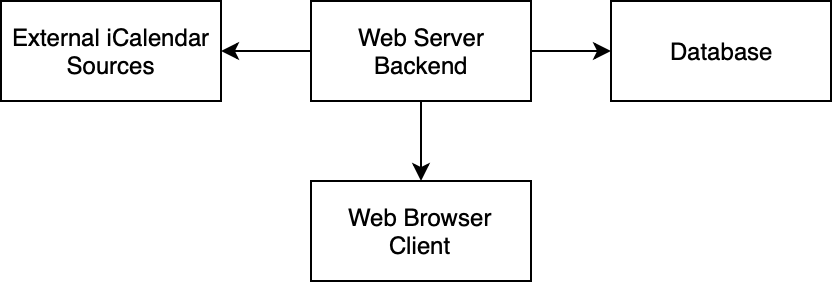
\includegraphics[width=1.0\textwidth]{systemDiagram}
    \caption{Environment Diagram}
    \label{fig:environment}
\end{figure}

\section{Design and Implementation Constraints}
For this system, our max performance and implementation is constrained by what
can be accomplished on the WSUV lab computers. As they are our targeted minimum,
going beyond their capabilities is not an option. We are also limited by our user
interface. As loading times are a priority in order to maximise usability, our
interface cannot be taxing to load on a moderate internet connection.

\section{User Documentation}
For the purpose of this application, a complete user manual is unnecessary.
Given the limited number of actions available to each User and simplicity of the
interface,the application should be able to be used by the User immediately,
provided the User is familiar with the scope of the application. For this
reason, a landing page with a brief description of the application, and an FAQ
page will be the extent of the User manual.

\section{Assumptions and Dependencies}
\begin{enumerate}
\item The system will rely on the .ical standardized calendar file format to
be imported from a preexisting calendar.
\item It is assumed a given Group will not exceed 50 members.
\item It is assumed a given User will not be a member of more than 50 Groups.
\end{enumerate}


\chapter{Specific Requirements}

\section{External Interface Requirements}
For the primary user interface, the User will be presented with a calendar view.
The calendar can be presented in either a monthly or weekly view. Along the left
edge of the calendar will be clickable tabs representing the different Groups
the User is a member of, which by clicking, the User can change which Group
focus they are interested in viewing. Along the right side will be similar tabs
representing the various Users and sub-Groups that are members of the same
Group that is selected. These tabs can be selected to filter out selected Users
from consideration. At the top right, the User can find links to manage their
settings and profile.
\section{Functional Requirements}

\subsection{User Management System}
    \begin{enumerate}
    \item The system shall allow non-Users to create accounts using a Username and password.
    \item The system shall allow Users to log in with their Username and password
    \item The system should allow Users to change their password
    \item The system should allow Users to change their Username
    \item The system should allow Users to delete their account
    \end{enumerate}

\subsection{Calendar Import System}
    \begin{enumerate}
    \item The system shall support importing calendars from Apple’s implementation of the iCalendar format.
    \item The system shall support importing calendars from Google’s implementation of the iCalendar format.
    \item The system should support importing calendars from arbitrary implementations of the iCalendar format.
    \item The system shall list the name and URL of the User’s previously imported calendars
    \item The system shall allow the User to remove a calendar from their profile
    \item The system should allow the User to manually refresh their calendars.
    \item The system will allow refreshing of calendars automatically as changes become available
    \end{enumerate}

\subsection{The Groups System}
    \begin{enumerate}
    \item The system shall allow Users to create Groups with a name and password.
    \item The system shall allow Group owners to issue invitations by a link.
    \item Non-Users who click an invite link will be directed to the registration page.
    \item After registering for an account through an invitation link, the system shall add the User to the Group.
    \item The system shall allow Users to join Groups by clicking an invitation link.
    \item The system shall allow Group owners to remove members from the Group.
    \item The system should allow Group owners to change the Group name and password.
    \item The system shall allow Group owners to delete a Group.
    \item The system will allow Group owners to leave a Group.
    \item The system shall not allow Group members to remove other members.
    \item The system shall allow Group members to leave a Group.
    \end{enumerate}

\subsection{The Calendar System}
    \begin{enumerate}
    \item The system shall allow the User to view time blocks that are available on a week-style view.
    \item When in week mode, the system shall allow the User to change the selected week forward or backward.
    \item The system shall allow the User to view time blocks that are available on a month-style view.
    \item When in month mode, the system shall allow the User to change the selected week forward or backward.
    \item The system shall allow the User to view time blocks that are available by selecting specific Users.
    \item The system will allow the User to view an aggregate set of time blocks from a selection Users and calendars.
    \item The system should treat events that are not marked `busy` as nonexistent and should consider them available.
    \end{enumerate}


\section{Behavior Requirements}

\begin{figure}[ht]
    \centering
    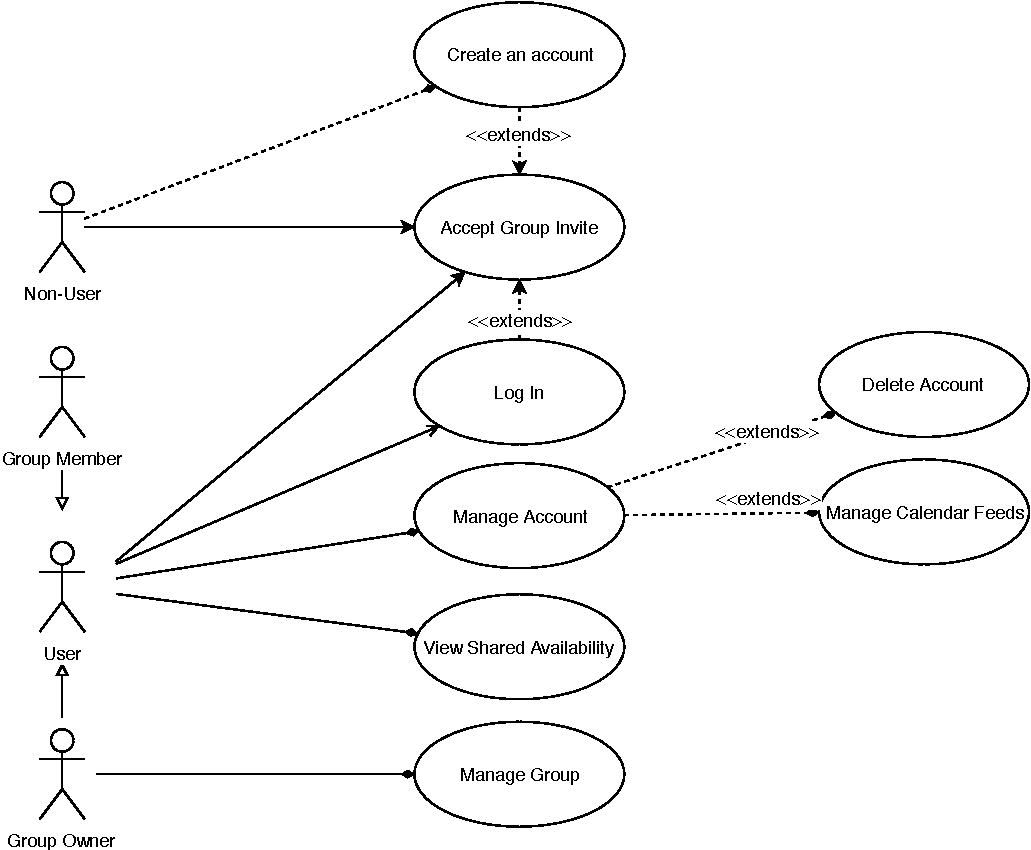
\includegraphics[width=1\textwidth]{CalendarProjectUseCases}
    \caption{Use Case Diagram}
    \label{fig:use-case}
\end{figure}

\begin{itemize}
\item Create Account - A New User without an account can create one.
\item Accept Group Invite - A User can accept a group invite from a Group Owner and be placed into a Group.
a New User will first be prompted to create an account.
\item Log in - A User with an account will be required to enter log-in information to acces the application.
\item Manage Account - A User can import and manage calendar files, view their Group memberships, and delete
their account.
\item Manage Calendar Feeds - A Group Member may select which Group they wish to view, and which Group
Members they wish to filter out.
\item View Shared Availability - A Group Member can view shared availability on the main calendar feed for a
selected Group they are a member of.
\item Manage Group - A Group Owner can change a Group name and password, invite Users and New Users to the
Group, and remove Group members from the Group.
\end{itemize}

\chapter{Nonfunctional Requirements}

\section{Performance Requirements}
\begin{enumerate}
\item Any action should not take more than 10 seconds to perform, assuming User
has a healthy internet connection.
\item The system should clearly identify when it is loading or processing
information with a loading indicator.
\item The system shall run without issue on Washington State University Vancouver
lab computers.
\end{enumerate}

\section{Safety and Security Requirements}
\begin{enumerate}
\item The system shall not access a User's calendar event names or descriptions,
only the dates and times of individual events.
\item The system shall not make any changes to a User's original calendar import,
only copy relevant information from the file into a simplified form.
\item The system shall not store a User's calendar file in any way, and shall
keep it only until the simplified file is created.
\end{enumerate}

\section{Software Quality Attributes}

\subsection{Reliability}
\begin{enumerate}
\item The system should be available 24/7 to the User, outside of scheduled maintenance
down times.
\item The system should be able to handle many concurrent Users without experiencing
usage interruptions.
\item Each Group should maintain full performance with 50 or less members.
\end{enumerate}

\subsection{Portability}
\begin{enumerate}
\item The system shall be fully usable on a desktop computer in a Google Chrome
browser.
\item The system should be usable on a desktop computer in other common browsers
such as Safari and Firefox.
\item The system will not support mobile accessibility.
\end{enumerate}

\subsection{Usability}
\begin{enumerate}
\item Most User functions should be accessible from the main page of the application,
without having to navigate through several pages.
\item The system should perform most of it's loading upon initial log-in, to allow
switching pages quickly without experiencing loading delays.
\end{enumerate}

\subsection{Interoperability}
\begin{enumerate}
\item The system shall accept calendar imports from the WSUV Blackboard calendar
format.
\item The system should accept calendar imports from other common calendar
applications.
\end{enumerate}

\chapter{Other Requirements}
The system will require use of a relatively small database. This database will be responsible for storing User profiles and Groups. The calendar files imported by the system will be highly condensed, so very little storage space will be needed.

\\\\The web application will conform to GDPR by allowing Users to delete their account and all their stored information from their profile screen.

\appendix

\chapter{Group Log}

\end{document}
